% Intended LaTeX compiler: pdflatex
\documentclass[10pt,a4paper,UTF8]{article}
\usepackage{zclorg}
\author{emacsun}
\date{}
\title{自学AI 和ML资料汇总}
\hypersetup{
 pdfauthor={emacsun},
 pdftitle={自学AI 和ML资料汇总},
 pdfkeywords={},
 pdfsubject={},
 pdfcreator={Emacs 25.0.50.1 (Org mode 9.0.5)}, 
 pdflang={English}}
\begin{document}

\maketitle
\tableofcontents
\titlepic{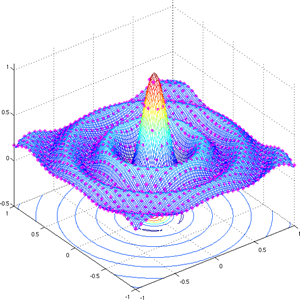
\includegraphics[scale=0.25]{../../img/sinc.PNG}}
\newpage

近年来,随着多个机器学习和人工智能项目的成功,机器学习和人工智能领域将会涌现出大量机会包括工作岗位和创业机会。因此,机器学习和人工智能将当之无愧的成为下一个风口。目前全国各地的科技城和产业园如雨后春笋般拔地而起,什么样的人才能够入住?以机器学习和人工智能技术为依托的互联网内容提供商将会占据很大比例。

处于这样一个飞速发展的时代,又恰好从事信息技术产业,对我来说没有什么是稳定的。等一切稳定,意味着没有机会。快速学习的技能将会是超越其他技能的最总要重要的技能。那么如何快速学习机器学习,本文提供了一些资料汇总。

\section{简介}
\label{sec:orgbcf2827}


机器学习是近20多年兴起的一门多领域交叉学科,涉及概率论、统计学、逼近论、凸分析、算法复杂度理论等多门学科。机器学习理论主要是设计和分析一些让计算机可以自动“学习”的算法。机器学习算法是一类从数据中自动分析获得规律,并利用规律对未知数据进行预测的算法。因为学习算法中涉及了大量的统计学理论,机器学习与统计推断学联系尤为密切,也被称为统计学习理论。算法设计方面,机器学习理论关注可以实现的,行之有效的学习算法。

\section{学习资料}
\label{sec:orgbf8c163}

\subsection{公开课}
\label{sec:org9dad3bd}


\begin{enumerate}
\item Andrew NG的《机器学习》,这个课程在网易公开课(据说版本比较老了),stanford学校上(cs229)还有coursera上也有的。
\item NTU 林轩田 《机器学习基石》和《机器学习技法》
\item corsera上明尼苏达两位老师的《Recommender system》
\item Caltech的公开课 learning from data
\end{enumerate}

\subsection{书籍}
\label{sec:org217f187}


\begin{enumerate}
\item 吴军 《数学之美》 科普用
\item 李航《统计学习方法》数学推导比较多
\item Harrington 《机器学习实践》调用了python的两个包numpy,scipy. scikit-learn几乎包含了所有常用的算法。
\item Duda 《模式分类》
\item 项亮的《推荐系统实践》
\item Kevin Murphy's \emph{\href{http://www.cs.ubc.ca/\~murphyk/MLbook/}{Machine learning: a Probabilistic Perspective}}
\item Hastie, Tibshirani, and Friedman's \emph{\href{http://statweb.stanford.edu/\~tibs/ElemStatLearn/}{The Elements of Statistical Learning}}
\item Bishop's \emph{\href{http://research.microsoft.com/en-us/um/people/cmbishop/prml/}{Pattern Recognition and Machine Learning}}
\item David Barber's \emph{\href{http://web4.cs.ucl.ac.uk/staff/D.Barber/pmwiki/pmwiki.php?n=Brml.HomePage}{Bayesian Reasoning and Machine Learning}}
\item Larry Wasserman's \emph{\href{http://www.amazon.com/All-Statistics-Statistical-Inference-Springer/dp/0387402721}{All of Statistics: A Concise Course in Statistical Inference}}
\item \emph{\href{http://www-bcf.usc.edu/\~gareth/ISL/}{An Introduction to Statistical Learning with Applications in R}}
\item Tom Mitchell的 machine learning,还有他的论文 \emph{The siscipline of Machine Learning}
\end{enumerate}
\subsection{博客}
\label{sec:org4ad0fea}


\begin{enumerate}
\item 林达华的博客
\item pluskid的博客
\item jerrylead 的博客
\item LeftNotEasy 的博客
\item Jason Brownlee的博客
\end{enumerate}
\subsection{资源汇总}
\label{sec:orgbb8d9c8}


\begin{enumerate}
\item \href{http://blog.jobbole.com/56256/}{机器学习的最佳入门学习资源} 系统总结了一些机器学习的相关资源。
\item \href{http://ml.memect.com/article/machine-learning-guide.html}{机器学习入门资源不完全汇总} 这里有相当详细的资源汇总,但是个人认为太过繁杂而有不成体系,看得头大
\item \href{https://www.zhihu.com/question/20691338}{机器学习该怎么入门} 张松阳的回答提供了比较多的有用资源
\item \href{https://github.com/josephmisiti/awesome-machine-learning/blob/master/books.md}{github awesome-machine-learning} 提供了不少资源,有书籍有项目,丰俭由人
\end{enumerate}

\section{学习方法}
\label{sec:org1203fd5}


读书,实践,读书,实践。

\begin{enumerate}
\item 有英文原版的尽量读英文原版。
\item 要有自己的项目输出(通过github来实现)
\item 要和别人有交流(通过github来实现)
\end{enumerate}
\section{学习日记}
\label{sec:org2ed6322}


这几天一直在看《linear algebra done right》和《Bayesian Reasoning and machine Learning》,同步学习的还有《Thinking in Java》以及《Python Doc》(这是Python的官方文档)。前两者是理论基础,后两者是工具。这与以后要从事的工作是高度契合的:既要懂得原理,又要会用计算机语言验证想法。

关于原理的学习还需要更输入的学习,接下来我的进一步计划是《随机过程》和《The Elements of Statistical Learning》。具体参阅哪一本书,稍后再定。不过在学习的过程中,一定要避免知识点的堆砌,所有的学习都要围绕一个问题展开来。为了保证这一点,我通过写博客的方式约束自己。每一篇博客都要有一个中心,围绕这个中心展开知识点的铺垫。中心就像树干,知识点的展开就像树枝,这样才有整体感。

\section{最重要的能力}
\label{sec:orgdf7eecf}


最重要的能力不是学习一门语言或者一种技术,最重要的能力是 \href{https://www.linkedin.com/pulse/20141113191054-103457178-the-only-skill-you-should-be-concerned-with?trk=mp-reader-card}{解决问题的能力} 。你所学习的语言,你所掌握的技术以及你的思维方式都是解决问题的副产品。所以不要为掌握了某种新技能沾沾自喜,解决问题的能力才是最重要的。

要有提问题的能力,提出问题,分析问题,搜集资料,解决问题。不要花费太多精力在搜集资料上,针对那些硬盘里放了一大堆电子书,并幻想自己已经掌握的硬盘式专家,我也不好多说什么。
\end{document}
